\cleardoublepage

\chapter{Mediciones y calibrado}
\label{makereference7}

\section{Mediciones de consumo}

El objetivo principal de Bluetooth Low Energy es incorporarse a dispositivos de bajo consumo, y ser lo más eficiente posible energéticamente. Por ello decidimos comprobar la eficiencia de consumo de energía de nuestra placa, conectándola a un osciloscopio y recogiendo los datos del amperaje durante la ejecución del programa, en el que se recogen los datos del acelerómetro, se envían por BLE y se entra en un estado de \textit{espera}. La gráfica resultante se muestra en la Figura~\ref{figuraConsumoMayo}.

\begin{figure}[h]%t=top, b=bottom, h=here
	\centering
    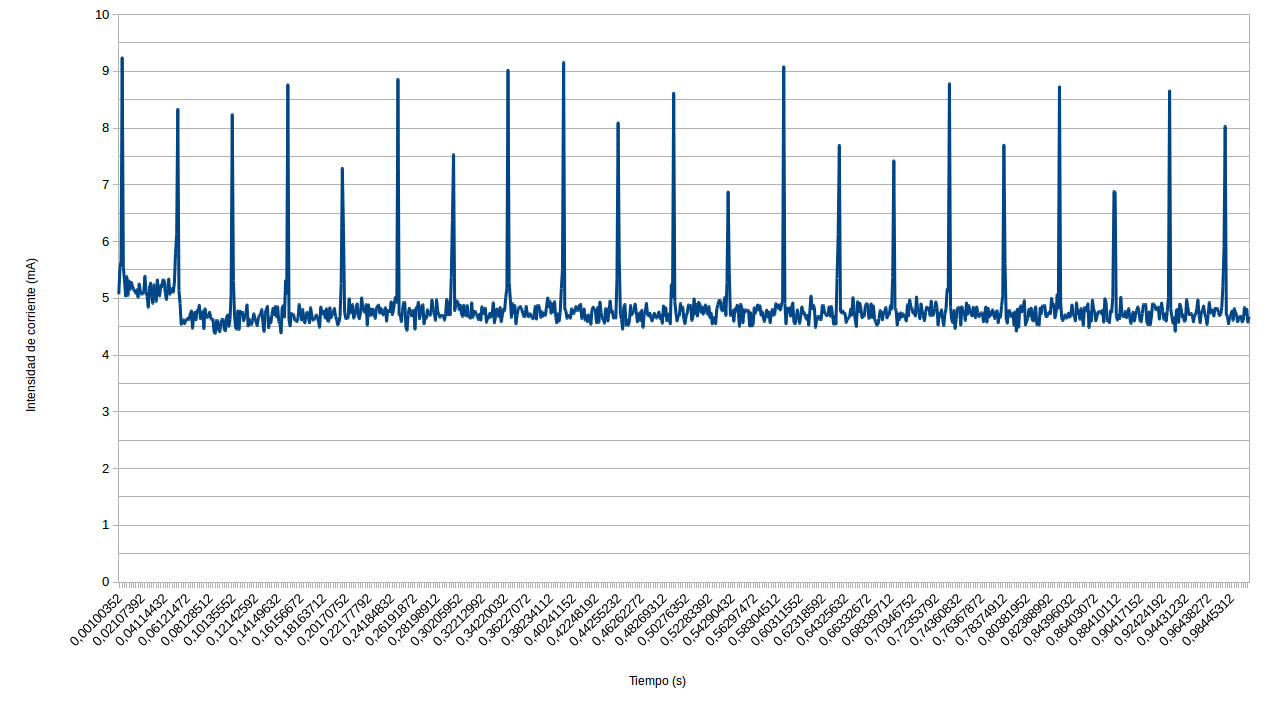
\includegraphics[width=\textwidth]{figures/consumo_mayo2.png}
    \caption[Primera gráfica de corriente]{Primera gráfica de corriente. Durante esta prueba el tiempo de espera estaba establecido en 0.1 s}
   	\label{figuraConsumoMayo}
\end{figure}

Se puede comprobar que no tiene un consumo muy elevado, con un máximo de 10 mA, que es cuando realiza la comunicación por BLE y un mínimo de cerca de 5 mA en los períodos inactivos. En los períodos de inactividad observamos que consume más de lo cabría esperar. Esto es debido a que pensábamos erróneamente que la función que utilizábamos para realizar la espera pondría al procesador en modo \textit{deep sleep}, que permitiría disminuir todo lo posible el uso de energía.

Buscando en la API de mbed, encontramos la forma de entrar en este modo, que se realiza con la función \textit{sleep( ms )}~\cite{APIDeepSleep}. Esta función ejecuta lo que se denomina un \textit{Wait for Interrupt}, que es una instrucción del repertorio de instrucciones de ARM que deja al procesador en modo de bajo consumo, parando todas las funcionalidades para ahorrar energía hasta que llegue una interrupción. La función \textit{sleep} que implementa la API de mbed determina dinámicamente en qué modo de bajo consumo se entrará.

El punto negativo de esto es que no hace discriminación entre los tipos de interrupción, por lo que puede salir del modo \textit{sleep} aunque no se lo hayamos indicado. Para evitar esto utilizamos un \textit{callback} que se ejecutará cada segundo, activando una variable booleana. Esta variable controla un bucle en el que, si sale del modo \textit{sleep} y no es por nuestra interrupción, vuelve a ejecutar un \textit{sleep}.

Una vez implementada esta funcionalidad, volvimos a realizar la prueba de consumo y esta vez obtuvimos resultados más satisfactorios, como se puede apreciar en la Figura~\ref{figuraConsumoJunio}.

\begin{figure}[h]%t=top, b=bottom, h=here
	\centering
    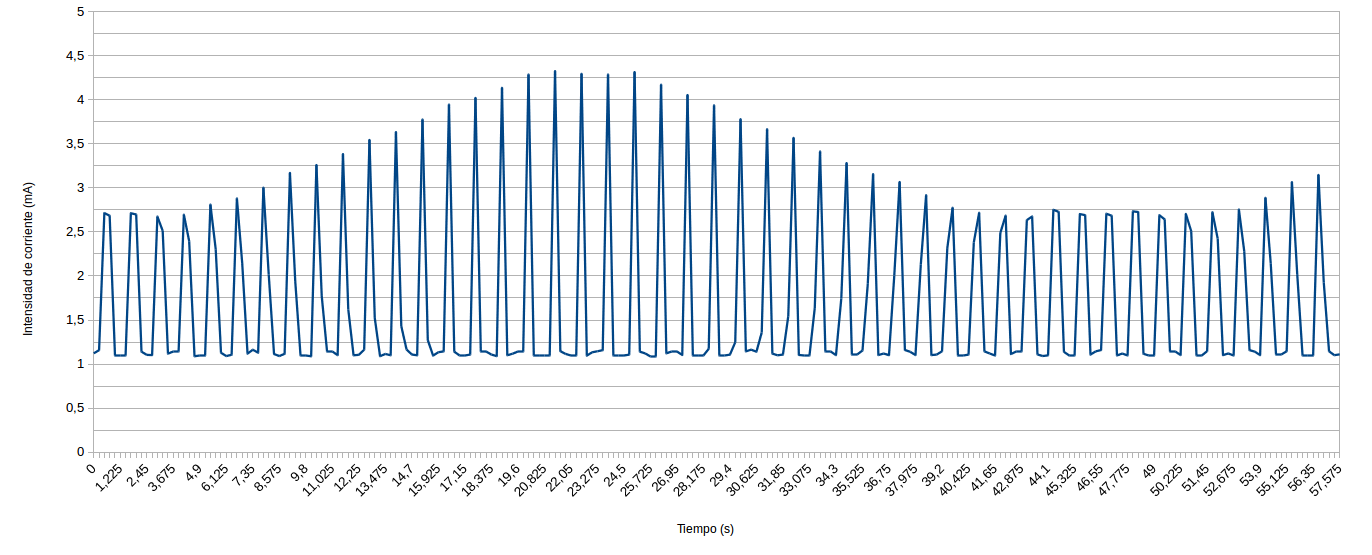
\includegraphics[width=\textwidth]{figures/consumo_junio2.png}
    \caption[Segunda gráfica de corriente]{Segunda gráfica de corriente. Cada segundo vemos un pico, que es cuando se despierta del sleep}
   	\label{figuraConsumoJunio}
\end{figure}

Como se puede ver, el consumo ha disminuido notablemente después de utilizar la función comentada, con mínimos en torno a 1.25 mA en los períodos de \textit{sleep}.

En estas pruebas observamos la existencia de unos picos de consumo cada 50 ms, que no se aprecian en la imagen ya que la recogida de datos se daba cada segundo. Estos picos se dan durante el período de bajo consumo, y sabemos que son debidos a la componente BLE puesto que realizamos pruebas con este módulo desactivado y no se presentaban, aunque no sabemos exactamente por qué se producen.

%% Cómo se calcularía el tiempo que nos puede durar la pila con los datos?

\section{Calibrado}

Para conocer qué rangos de los datos de acelerometría podían ser interesantes para representarlos en la ruta, realizamos una serie de pruebas para obtener valores reales y luego los analizamos para sacar conclusiones. Pronto nos dimos cuenta de que dependiendo de la posición en la que se encuentre nuestro dispositivo, los resultados pueden variar en gran medida. Por lo que sería necesario un proceso de calibración antes de empezar la marcha.

Para nuestro proyecto, nos hemos centrado en el eje x para determinar la aceleración en cada momento. Decidimos establecer una serie de umbrales para colorear la ruta en el mapa generado, de modo que si detectamos un valor negativo, es decir, una deceleración, usamos el color azul. Si estamos en un valor cercano a 0, usamos el verde. En cuanto aceleramos ligeramente (hasta los 100 mg), usamos el amarillo, y a partir de ahí cuando se acelera aún mas usamos el rojo.

Debido a la presencia constante de la aceleración de la gravedad en cualquier objeto, el acelerómetro recoge siempre este valor, repartido entre los ejes (x, y, z). En llano, la aceleración o deceleración se produce sólo en el eje x, pero cuando nos hallamos en una pendiente este valor se reparte entre los ejes (x, z), por lo que parte de la aceleración se juntará con el valor de la gravedad.

\cleardoublepage

\chapter{Conclusiones y trabajo futuro}
\label{makereference8}

Este proyecto nos ha permitido explorar tecnologías hardware con las que no habíamos trabajado nunca, como Bluetooth Low Energy y protocolos como SPI o I2C, lo que nos ha dado unas competencias en otros campos que no son específicamente los nuestros. Hemos aprendido a programar una placa desde cero, investigando la documentación que pone a nuestra disposición el fabricante y encontrando ejemplos para lograr los objetivos propuestos.

En el campo del desarrollo software, hemos trabajado por primera vez en el desarrollo de una aplicación Android, familiarizándonos con el entorno de programación \textit{Android Studio}.

La línea de aprendizaje que hemos recorrido (en la que hemos empezado haciendo numerosas pruebas pequeñas antes de continuar con el proyecto final) nos ha permitido empezar por conceptos sencillos y fáciles de entender que nos permitían avanzar rápidamente a casos mas complejos.

Finalmente, hemos logrado producir una aplicación que se puede utilizar en entornos reales, con la que, fijando la placa BLE en una bicicleta, podemos realizar una ruta y visualizar correctamente los datos generados durante la misma.

Bluetooth Low Energy es un concepto muy interesante, y abre las puertas para comunicar gran cantidad de dispositivos. Con esta tecnología podríamos realizar más proyectos útiles que hasta ahora no eran posibles.

\section{Trabajo futuro}

Aunque la aplicación es funcional y cumple con los requisitos del proyecto, siempre es interesante la idea de ampliar la utilidad de nuestra aplicación.

Un ejemplo claro es el de poder aprovechar aún más el hecho de tener la aplicación ejecutándose en un dispositivo móvil, ofreciendo la posibilidad de compartir las sesiones realizadas en las redes sociales (Twitter, Facebook, ...).

Otra posibilidad que sería de utilidad es la de fijar una luz de freno a la placa, que al detectar una deceleración se encienda para indicar a conductores, peatones, etc. que se está reduciendo la velocidad para evitar accidentes.

En relación con esto, otro punto importante de cara al futuro es el de utilizar los datos que se recogen de acelerometría para comprobar movimientos muy bruscos (como los que se darían en caso de accidente) para activar un sistema que avise a los servicios de emergencia en caso de que el usuario no responda en un breve tiempo.

Se podrían realizar más cálculos con los datos obtenidos para poder sacar más información de la ruta. Además, aprovechando que la placa XTRINSIC-SENSE-BOARD contiene, aparte del acelerómetro que usamos, un magnetómetro y un sensor de presión, se podría recoger mucha más información sobre el esfuerzo realizado durante el trayecto.

